%%%%%%%%%%%%%%%%%%%%%%%%%%%%%%%%%%%%%%%%%%%%%%%%%%%%%%%%%%%%%%%%%%%%%%%%%%%%%%%%
% Diese Datei beinhaltet den eigentlichen Inhalt Ihrer Arbeit.
%
% Es bietet sich der Übersicht halber an, die einzelnen Abschnitte jeweils
% in eigene Dateien zu schreiben und mittels \input einzubinden.
% Eine mögliche Verzeichnisstruktur sähe entsprechend so aus:
%
%     thesis/
%     +- tex/
%     |  +- introduction.tex
%     |  +- motivation.tex
%     |  +- experiments.tex
%     |  |  ...
%     |  +- conclusion.tex
%     +- abstract.tex
%     +- contents.tex
%     +- thesis.tex
%%%%%%%%%%%%%%%%%%%%%%%%%%%%%%%%%%%%%%%%%%%%%%%%%%%%%%%%%%%%%%%%%%%%%%%%%%%%%%%%

\section{Einleitung}

Dies ist der Hauptteil Ihrer Arbeit.
In der Datei \texttt{references.bib} finden Sie bereits einige Quellen,
die Sie wahrscheinlich zitieren mögen,
wie z.B. die B Methode~\cite{abrial1996b,abrial2010modeling}
oder \textsc{ProB}~\cite{leuschel2003prob,leuschel2008prob}.
Beachten Sie den Artikel ``Common Errors in Bibliographies'' von John Owens.%
\footnote{\url{https://www.ece.ucdavis.edu/~jowens/biberrors.html}}

\cref{sec:figures,sec:tables}
geben je ein kurzes Beispiel,
wie Bilder bzw. Tabellen in \LaTeX{} erstellt werden.
\cref{sec:plot} zeigt die Einbindung eines Graphen.


\subsection{Makefile}

Im Wurzelverzeichnis finden Sie ein \texttt{Makefile}.
Über das Terminal können Sie die folgenden Befehle aufrufen:


\begin{tabularx}{\textwidth}{lX}
  \toprule
  \texttt{make} & Kompiliert das PDF und löscht aux-Files. \\
  \texttt{make clean} & Löscht das PDF und dazugehörige aux-Files. \\
  \texttt{make bibtool} & Sortiert \texttt{references.bib}
  und formatiert die Einträge einheitlich. \\
  \texttt{make watch} & Rekompiliert das PDF bei Änderungen und
  hält die Anzeige in Ihrem PDF-Betrachter aktuell. \\
  \bottomrule
\end{tabularx}

\section{Notizen}%
\subsection{Bytecode}

Um die VM Cache-Effizient und damit schnell zu halten, ist es wichtig, ein günstiges Format für den internen Bytecode zu finden.
Ein Enum zu benutzen, würde bewirken, dass zur Laufzeit alle Instruktionen die selbe Größe hätten. Dies wäre jedoch nicht sinnvoll, da nur manche Instruktionen Parameter benötigen.
Es wäre eine Verschwendung von Arbeitsspeicher, wenn simple Add-Instruktionen die gleiche Größe hätten wie Call-Instruktionen.

Somit macht es Sinn, Instruktionen mit verschiedenen Größen zu verwenden. Die VM konsumiert eine Instruktion und dann abhängig von dieser eine beliebige Anzahl an Parametern.
Im Code ist dies mit einer Kombination aus Enums und Unions umgesetzt. Opcode ist ein Union, welches entweder eine Instruktion, ein Segment oder einen Acht-Bit Konstante sein kann. Die beiden Enums Instruction und Segment sind jeweils auch durch ein einziges Byte kodiert.

\begin{lstlisting}
  #[repr(u8)]
  pub enum Segment {
    Argument = 0,
    Local = 1,
    // ...
  }

  #[repr(u8)]
  pub enum Instruction {
    Add = 0,
    Sub = 1,
    // ...
  }

  #[repr(C)]
  pub union Opcode {
    instruction: Instruction,
    segment: Segment,
    constant: u8,
  }
\end{lstlisting}

Mit diesem System verbrauchen Instruktionen nur genau soviel Speicher wie notwendig, was eine effizientere Cache-Auslastung und somit bessere Performance ermöglicht.

\subsection{Parsing}
Da die Anwendung eine Reihe an Parsern enthält, macht es Sinn gemeinsame Komponenten auszulagern.

\subsection{Keyboard}
Das Keyboard handling ist eine Übersetzung des entsprechenden Java Codes in der offiziellen Implementierung.
Zunächst wurde dies in Javascript implementiert, jedoch war zu diesem Zeitpunkt schon eine Portierung in den Rust Code geplant.
Die Verarbeitung von Sonderzeichen, wie Backspace oder Enter ist in Javascript anders als in Java, da diese als String im Event stehen.

\subsection{Fehlerhafte Auflösung lokaler Symbole}
VM crashed bei mehreren Beispielen

Das Problem war eine falsche Kompilierung von Labels. Die erste Implementierung hatte nur eine Symboltabelle für lokale und globale Symbole, welche nie zurückgesetzt wurde. Dies führt jedoch zu einer Reihe von Problemen.
Jump Instruktionen können zu Labels springen, welche weiter unten im Quellcode stehen und somit der Symboltabelle noch nicht bekannt waren. Dies wurde möglich indem anstatt einer Instruktion, ein Platzhalterwert benutzt wurde, welcher später durch die tatsächliche Instruktion ersetzt wurde.
Allerdings hatte dieses Verfahren ohne weitere Anpassungen ein Problem, wenn der Jack Compiler das selbe Label in verschiedenen Prozeduren verwendet. Da die Symboltabelle nie zurückgesetzt wurde, hat der Parser das Label nicht als noch unbekannt identifiziert, sonder hat stattdessen einen Jump in eine vorherige Funktion produziert.
Um dieses Problem zu beheben, erhält nun jede Funktion ihre eigene Symboltabelle


\subsection{Memory corruption in Tetris}
Wenn man in meiner Projekt 9 Abgabe einen gedrehten Stein an den rechten Rand bewegt, stürzt das Spiel ab. Dies passiert nicht im offiziellen Emulator, was mich vermuten lässt, dass Speicher überschrieben wird, welcher von der Stdlib benutzt wird. Dieser Absturz findet in der offiziellen Implementierung auch statt, allerings nur wenn man die Bytecode implementierung der Stdlib verwendet, nicht aber mit der eingebauten Java Implementierung.


\section{Bilder und Co.}

\subsection{Bilder}%
\label{sec:figures}

In \cref{fig:initial-draft} ist festgehalten,
wie alles angefangen hat.


\subsection{Tabellen}%
\label{sec:tables}

\cref{table:truths} fasst die Wahrheiten dieser Welt zusammen.

\begin{table}[ht]
  \begin{center}
    \begin{tabular}{lr}
      \toprule
      Fakt                                & Wahrheitsgehalt \\
      \midrule
      booktabs Tabellen sind hübscher     & 90 \%           \\
      Han Solo schoss zuerst              & 100 \%          \\
      Game of Thrones fand ein gutes Ende & 0 \%            \\
      \bottomrule
    \end{tabular}
    \caption{Table of truths.}%
    \label{table:truths}
  \end{center}
\end{table}

\subsection{Plots}%
\label{sec:plot}

Sie können mithilfe von \texttt{tikz} und \texttt{pgfplots}
ganz leicht Graphen erstellen:

\begin{figure}[ht]
  \centering
  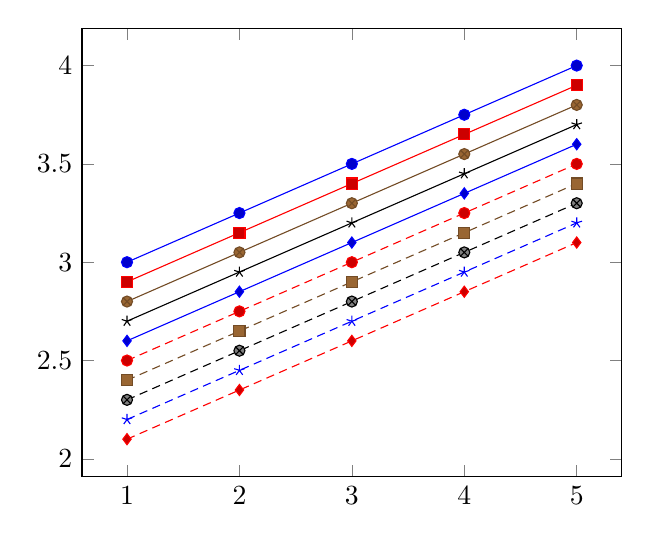
\begin{tikzpicture}
    \begin{axis}
      \foreach \y in {0,0.1,...,1} % Wiederholt \addplot mit jeweils anderem \y
        \addplot coordinates {
            ( 1, 3.0 -\y)
            ( 2, 3.25-\y)
            ( 3, 3.5 -\y)
            ( 4, 3.75-\y)
            ( 5, 4.0 -\y)
          };
    \end{axis}
  \end{tikzpicture}
  \caption{A beautiful plot.}%
  \label{fig:the-plot}
\end{figure}

\section{Conclusion}

Am Ende der Arbeit werden noch einmal die erreichten Ergebnisse
zusammengefasst und diskutiert.
